\documentclass[12pt,a4paper]{article}


\usepackage%
	[%
	paper=a4paper,%
	top=0.75cm,headheight=0.3cm,headsep=0.5cm,%
	bottom=2cm,footskip=1cm,%
	left=1.5cm,right=1.5cm%
	]%
	{geometry}

\usepackage{color}
\definecolor{verylightgray}{gray}{.9}
\definecolor{lightgray}{gray}{.8}
\definecolor{gray}{gray}{.7}
\definecolor {brown} {rgb} {0.74, 0.30, 0.12}
\definecolor {orange} {rgb} {1, 0.50, 0}
\definecolor {darkgreen} {rgb} {0, 0.9, 0}
\definecolor {lightblue} {rgb} {0.5, 0.5, 1}
\definecolor {bordeaux} {cmyk} {0, 0.735, 0.270, 0.257}

%\usepackage{textcomp}

\usepackage{url}

\usepackage{graphics}
\graphicspath{{./}}

\usepackage {listings}

%\definecolor{codegreen}{rgb}{0,0.8,0}
\definecolor{codeblue}{rgb}{0,0,0.9}
\definecolor{codegreen}{rgb}{0,0.4,0}
\definecolor{codegray}{rgb}{0.5,0.5,0.5}
\definecolor{codepurple}{rgb}{0.58,0,0.82}
\definecolor{backcolour}{rgb}{0.95,0.95,0.92}
%\definecolor{backcolour}{rgb}{0.97,0.97,0.94}
 
\lstdefinestyle{mystyle}{
	frame=shadowbox, framesep=3pt, rulesep=2pt, rulesepcolor=\color{orange}, 
  %backgroundcolor=\color{backcolour},   
  commentstyle=\color{codeblue},
  keywordstyle=\color{magenta},
  %numbers=left,
  numberstyle=\tiny\color{codegray},
  stringstyle=\color{codepurple},
  basicstyle=\ttfamily\footnotesize,
  breakatwhitespace=false,         
  breaklines=true,                 
  captionpos=t,      % top               
  keepspaces=true,                 
  numbers=left,                    
  numbersep=5pt,                  
  showspaces=false,                
  showstringspaces=false,
  showtabs=false,                  
  tabsize=2
} 
\lstset{style=mystyle}


\newcommand{\mxml}{MusicXML}

\newfont\pnt{pzdr at 24.88pt}
\newcommand{\hand}[1]{
  \makebox[0pt][r]{
  	\textcolor{bordeaux}{\raisebox{-.5ex}{\pnt\symbol{'345}}}\hspace{1em}
	}%
	\hfill%
	{%
	  \setlength{\fboxsep}{2ex}%
	  \colorbox{white}{
	  	\parbox{.8\textwidth}{\textcolor{bordeaux}{\textbf{#1}}}
	  }
		\hfill
	}
}

\setlength {\parindent} {0mm}

\setlength {\parskip} {2.8ex plus \baselineskip minus 2pt}

% -------------------------------------------------------------------------
\begin{document}
% -------------------------------------------------------------------------

%\noindent

\title{
Introduction to \mxml\\[5pt]
\small {Notensatz-Konferenz, Salzburg Mozarteum, January 17-18, 2019}
}

\author{
Jacques Menu \footnote {Former lecturer in computer science at Centre Universitaire d'Informatique, University of Geneva, Switzerland}
}

\date {DRAFT -- \today}
%\date {}

\maketitle

\abstract {
This document presents a basic view of \mxml\ and a couple of short examples illustrating how \mxml\ represents a music score. Our goal is to give a flavor of what \mxml\ definitions and data look like from a musician's point of view.

All the examples mentioned can be downloaded from \url{https://github.com/grame-cncm/libmusicxml/tree/lilypond/files/samples/musicxml}. They are grouped by subject in subdirectories, such as '{\tt basic/HelloWorld.xml'}.

The scores fragments shown in this document have been produced by translating the {'\tt .xml}' files to LilyPond syntax, and then creating the graphical score with LilyPond. The translations have been done by {\tt xml2ly}, a prototype tool developed by this author. {\tt xml2ly} and these examples are this author's contribution to {\tt libmusicxml2}, an open-source C++ library created and maintained by Dominique Fober at Grame, Lyon, France. The home page to {\tt libmusicxml2} is \url{https://github.com/grame-cncm/libmusicxml}.

The reader can handle the {'\tt .xml}' file examples with their own software tools to compare the results with the ones herein.
}

% -------------------------------------------------------------------------
% -------------------------------------------------------------------------
\section{Overview of \mxml\ }
% -------------------------------------------------------------------------
% -------------------------------------------------------------------------

% -------------------------------------------------------------------------
\subsection{What \mxml\ is}
% -------------------------------------------------------------------------

\mxml\ ({\it Music eXtended Markup Language}) is a specification language meant to represent music scores by texts, readable both by humans and computers. It has been designed by the W3C Music Notation Community Group to help sharing music score files between applications, through export and import commands mechanisms.

The homepage to \mxml\ is \url{https://www.musicxml.com}.

\mxml\ data contains very detailed information about the music score, and is quite verbose by nature. This makes creating such data quite difficult by hand, but this should be done by applications actually.

% -------------------------------------------------------------------------
\subsection{\mxml\ formal definition}
% -------------------------------------------------------------------------

As a member of the *XML family of languages, \mxml\ is defined by a DTD ({\it Document Type Definition}), to be found at \url{https://github.com/w3c/musicxml/tree/v3.1}. 

The '{\tt schema}' subdirectory contains '{\tt *.mod}' text files defining the various concepts. {'\tt common.mod}' contains definitions used in other {'\tt *.mod}' files.

For example, here is how the '{\tt backup}' and {\tt forward}' markups:
\begin{lstlisting}[language=XML, caption=$<$backup$>$ and $<$forward$>$ example]
      <forward>
        <duration>4</duration>
        <voice>2</voice>
        <staff>1</staff>
      </forward>
      <backup>
        <duration>8</duration>
      </backup>
\end{lstlisting}

are defined in '{\tt note.mod}':
\begin{lstlisting}[language=XML, caption=$<$backup$>$ and $<$forward$>$ definition]
<!--
	The backup and forward elements are required to coordinate
	multiple voices in one part, including music on multiple
	staves. The forward element is generally used within voices
	and staves, while the backup element is generally used to
	move between voices and staves. Thus the backup element
	does not include voice or staff elements. Duration values
	should always be positive, and should not cross measure
	boundaries or mid-measure changes in the divisions value.
-->
<!ELEMENT backup (duration, %editorial;)>
<!ELEMENT forward
	(duration, %editorial-voice;, staff?)>
\end{lstlisting}

The current \mxml\ DTD version is 3.1, and there are discussions about version 3.2.

The syntactical aspects of \mxml\ are quite simple and regular, which makes it easy to handle these aspects with algorithms.

It is very difficult though to define the semantics -- the meaning of the sentences -- of an artificial language in a complete and consistent way, i.e. without omitting anything and without contradictions. \mxml\ is no exception to this rule, and there are things unsaid in the DTD, which leaves room to interpretation by the various applications that create or handle \mxml\ data.

% -------------------------------------------------------------------------
\subsection{Part-wise vs. measurewise descriptions}
% -------------------------------------------------------------------------

\mxml\ allows the score to be represented as a sequence of parts, each containing a sequence of measures, or as a sequence of measures, each containing a sequence of parts, i.e. data describing the contents of the corresponding measure in a part.
 
It seems that measure-wise descriptions have been very little used, and we shall stick to part-wise \mxml\ data in this document.

As a historical note, an XSL/XSLT script was supplied in the early days of \mxml\ to convert between part-wise and measure-wise representations.

% -------------------------------------------------------------------------
\subsection{Markups}
% -------------------------------------------------------------------------

\mxml\ data is made of so-called markups, composed of two parts. The opener is introduced by a '{\tt <}' and closed by a '{\tt >}', as in '{\tt <part-list>}'. The closer and second part is introduced by a '{\tt </}' and closed by a '{\tt >}', as in '{\tt </part-list>}'.

Markups can be self sufficient, as the example above, or go by pairs, which allows nesting markups, such as:
\begin{lstlisting}[language=XML]
        <duration>4</duration>
\end{lstlisting}
and:
\begin{lstlisting}[language=XML]
        <clef>
          <sign>G</sign>
          <line>2</line>
        </clef>
\end{lstlisting}

Markups can have attributes such as the part name '{\tt P1}' in:
\begin{lstlisting}[language=XML]
        <score-part id="P1">
          <part-name>Music</part-name>
        </score-part>
\end{lstlisting}
Some such attributes are mandatory such as {'\tt id}' in {'\tt score-part}', while others are optional.

It is possible to contract an element that contains nothing between its opener and closer, such as:
\begin{lstlisting}[language=XML]
        <dot></dot>
\end{lstlisting}
this way:
\begin{lstlisting}[language=XML]
        <dot />
\end{lstlisting}

Comments can be used in \mxml\ data. They start with {'\tt <!--}' and end with {'\tt -->}', as in:
\begin{lstlisting}[language=XML]
<!--=========================================================-->
    <measure number="1">
  <!-- A very minimal MusicXML example, part P1, measure 1 -->
\end{lstlisting}

Comments can span several lines.

The spaces and end of lines between markups are ignored.

\hand {\mxml\ is a representation of HOW TO DRAW a score, which has implications on the kind of markups available, in particular {'\tt <forward>}' and {'\tt <backup>}', which are presented at section \ref{forwardAndBackup} %\ContentsPageLink{NAT}{à la}.
}

Markups are called {'\tt elements}' in the \mxml\ DTD, and we shall use that terminology in the remainder of this paper.

% -------------------------------------------------------------------------
\subsection{Overall structure}
% -------------------------------------------------------------------------

\mxml\ data consists of:
\begin{itemize}
\item a {'\tt <?xml>}' element indicating the characters encoding used;
\item a {'\tt <!DOCTYPE>}' element telling that the data below is in {'\tt score-partwise}' mode; 
\item a {'\tt <score-partwise>}' element indicating the \mxml\ DTD number that the forthcoming data complies to, and that contains:

\begin{itemize}
\item a {'\tt <part-list>}' element containing the various {'\tt <score-part>}'s in the score;
\item a sequence of {'\tt <part>}' elements in the order they appear in the score, each one containing the measures in the given part, in order. 
\end{itemize}

\end{itemize}


% -------------------------------------------------------------------------
% -------------------------------------------------------------------------
\section{A complete example}
% -------------------------------------------------------------------------
% -------------------------------------------------------------------------

As is usual in computer science, this example is named '{\tt basic/HelloWorld.xml'}. It is displayed below, together with the resulting graphic score.

The first line specifies the character encoding of the contents below, here UTF-8. Then the '{\tt !DOCTYPE}' element at lines 2 to 4 tells us that this file contains partwise data conforming to DTD 3.0.

Then the '{\tt <part-list>}' element at lines 7 to 11 contains a list of '{\tt <score-part>}'s with their '{\tt id}' attribute, here '{\tt P1}' alone.

After this, we find the sequence of '{\tt part}'s with their '{\tt id}' attribute, here '{\tt P1}' alone, and, inside it, the single '{\tt <measure>}' element with attribute '{\tt number}' 1.

The nesting of elements, such as {'\tt <key>}' containing a {'\tt <fifths>}' element, leads the structure of a \mxml\ representation to be a tree. The way the specification is written conforms to the computer science habit of drawing trees with their root at the top and their leaves at the bottom.

%\begin{figure}
%\caption{Contents of {'\tt basic/Helloworld.xml}'}\label{helloworld}
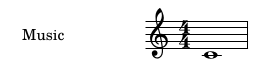
\includegraphics{HelloWorld.png}

\begin{lstlisting}[language=XML, caption =HelloWorld.xml]
<?xml version="1.0" encoding="UTF-8" standalone="no"?>
<!DOCTYPE score-partwise PUBLIC
    "-//Recordare//DTD MusicXML 3.0 Partwise//EN"
    "http://www.musicxml.org/dtds/partwise.dtd">
<score-partwise version="3.0">
  <!-- A very minimal MusicXML example -->
  <part-list>
    <score-part id="P1">
      <part-name>Music</part-name>
    </score-part>
  </part-list>
  <part id="P1">
<!--=========================================================-->
    <measure number="1">
  <!-- A very minimal MusicXML example, part P1, measure 1 -->
      <attributes>
        <divisions>1</divisions>
        <key>
          <fifths>0</fifths>
        </key>
        <time>
          <beats>4</beats>
          <beat-type>4</beat-type>
        </time>
        <clef>
          <sign>G</sign>
          <line>2</line>
        </clef>
      </attributes>
  <!-- A very minimal MusicXML example, part P1, measure 1, before first note -->
      <note>
        <pitch>
          <step>C</step>
          <octave>4</octave>
        </pitch>
        <duration>4</duration>
        <type>whole</type>
      </note>
    </measure>
<!--=========================================================-->
  </part>
</score-partwise>
\end{lstlisting}
%\end{figure}

% -------------------------------------------------------------------------
% -------------------------------------------------------------------------
\section{Top-level structure}
% -------------------------------------------------------------------------
% -------------------------------------------------------------------------

% -------------------------------------------------------------------------
\subsection{Part groups and parts}
% -------------------------------------------------------------------------

Part groups are used to structure complex scores, mimicking the way large orchestras are organized. For example, there can be a winds group, containing several groups such as flutes, oboes, horns and bassoons.

The \mxml\ DTD state that part groups me be interleaved.

% -------------------------------------------------------------------------
\subsection{Staves and voices}
% -------------------------------------------------------------------------

There's no staff or voice component as such in \mxml\ data: one knows they exist because they are mentioned in notes and other elements, such as:
\begin{lstlisting}[language=XML]

\end{lstlisting}

% -------------------------------------------------------------------------
% -------------------------------------------------------------------------
\section{Staff and voice level}
% -------------------------------------------------------------------------
% -------------------------------------------------------------------------

% -------------------------------------------------------------------------
\subsection{Clefs}
% -------------------------------------------------------------------------

 

% -------------------------------------------------------------------------
\subsection{Keys}
% -------------------------------------------------------------------------

 

% -------------------------------------------------------------------------
\subsection{Time signatures}
% -------------------------------------------------------------------------

 

% -------------------------------------------------------------------------
\subsection{Measures}
% -------------------------------------------------------------------------

Anacruses 

% -------------------------------------------------------------------------
\subsection{Numbering}
% -------------------------------------------------------------------------

The various parts in a (part-wise) \mxml\ descriptions are usually named from '{\tt P1}' on, but any name could be used.

Measures are usually numbered from {'\tt 1}' up, but these numbers are actually character strings, not integers: this allows for special measure numbers such as {'\tt X1}', for example, in the case of cue staves.

Staves have numbers from {'\tt 1}' up, with stave number {'\tt 1}' the top-most one in a given part.

% -------------------------------------------------------------------------
% -------------------------------------------------------------------------
\section{Measurements}
% -------------------------------------------------------------------------
% -------------------------------------------------------------------------

% -------------------------------------------------------------------------
\subsection{Geometrical lengths}
% -------------------------------------------------------------------------

\mxml\ represents lengths by 10$^{th}$ of in interline space, i.e. the distance between lines in staves. This relative measure unit has the advantage that if does not change if the score is scaled by some factor.

In {'\tt common.mod}' we find:

\begin{lstlisting}[language=XML]
}
<!--
	The tenths entity is a number representing tenths of
	interline space (positive or negative) for use in
	attributes. The layout-tenths entity is the same for
	use in elements. Both integer and decimal values are 
	allowed, such as 5 for a half space and 2.5 for a 
	quarter space. Interline space is measured from the
	middle of a staff line.
-->
<!ENTITY % tenths "CDATA">
<!ENTITY % layout-tenths "(#PCDATA)">
\end{lstlisting}

In order to obtain absolute lengths, \mxml\ specifies how many tenths there are equal to how many millimeters in the {'\tt <scaling>}' element, defined in {'\tt layout.mod}':

\begin{lstlisting}[language=XML]
<!--
	Version 1.1 of the MusicXML format added layout information
	for pages, systems, staffs, and measures. These layout
	elements joined the print and sound elements in providing
	formatting data as elements rather than attributes.

	Everything is measured in tenths of staff space. Tenths are
	then scaled to millimeters within the scaling element, used
	in the defaults element at the start of a score. Individual
	staves can apply a scaling factor to adjust staff size.
	When a MusicXML element or attribute refers to tenths,
	it means the global tenths defined by the scaling element,
	not the local tenths as adjusted by the staff-size element.
-->
\end{lstlisting}
\dots \dots \dots \dots \dots \dots
\begin{lstlisting}[language=XML]
<!--
	Margins, page sizes, and distances are all measured in
	tenths to keep MusicXML data in a consistent coordinate
	system as much as possible. The translation to absolute
	units is done in the scaling element, which specifies
	how many millimeters are equal to how many tenths. For
	a staff height of 7 mm, millimeters would be set to 7
	while tenths is set to 40. The ability to set a formula
	rather than a single scaling factor helps avoid roundoff
	errors.
-->
<!ELEMENT scaling (millimeters, tenths)>
<!ELEMENT millimeters (\#PCDATA)>
<!ELEMENT tenths %layout-tenths;>
\end{lstlisting}

This leads for example to:
\begin{lstlisting}[language=XML, caption=Scaling example]
        <scaling>
          <millimeters>7.05556</millimeters>
          <tenths>40</tenths>
        </scaling>
\end{lstlisting}

% -------------------------------------------------------------------------
\subsection{Notes durations}
% -------------------------------------------------------------------------

\mxml\ uses a quantization of the duration with the {'\tt <divisions>'} element, which tells how many divisions there are in a quarter note:
\begin{lstlisting}[language=XML]
       <divisions>2</divisions>
\end{lstlisting}

This example means that there are 2 division in a quarter note, i.e. the duration measure unit is an eigth note. Let's borrow from physics and MIDI terminology and call this a quantum.

Any multiple of this quantum can be used in the \mxml\ data after that specification, but there's no way to express a duration less than an eigth node.

The quantum value has to be computed from the shortest note in the music that follows this element, taking tuplets into account, see below. 

Is it possible to set the quantum to other values later in the \mxml\ data at will if needed? The DTD doesn't mentions that, and in practice, all applications support this feature.

% -------------------------------------------------------------------------
% -------------------------------------------------------------------------
\section{Note level}
% -------------------------------------------------------------------------
% -------------------------------------------------------------------------

A note is described by a {'\tt note}' element, such as this snippet from {'\tt basic/MinimalScore.xml}':

\begin{lstlisting}[language=XML, caption =Note example]
        <divisions>8</divisions>
        
      <!-- ... ... ... ... ... -->
      
        <clef>
          <sign>G</sign>
          <line>2</line>
          <clef-octave-change>-1</clef-octave-change>
        </clef>

      <!-- ... ... ... ... ... -->
      
      <note>
        <pitch>
          <step>E</step>
          <alter>-1</alter>
          <octave>4</octave>
        </pitch>
        <duration>28</duration>
        <voice>1</voice>
        <type>half</type>
        <dot />
        <dot />
        <accidental>flat</accidental>
      </note>
\end{lstlisting}

This is the first note in measure 2 of:\\
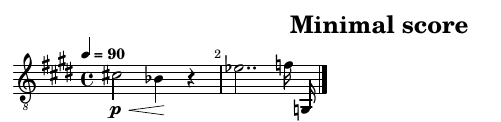
\includegraphics{MinimalScore.png}

In this example, the various sub-elements are:
%\begin{adjustwidth}{-0.5cm}{-0.5cm}
\begin{center}
\footnotesize
\def \contentsWidth{0.5\textwidth}
\def \arraystretch{1.3}
%
\begin{tabular}[t]{lp{\contentsWidth}}
\textbf{Fragment}&\textbf{Meaning} \tabularnewline[0.5ex]
\hline\\[-3.0ex]
%
{'\tt <step>E</step>}' & the diatonic pitch of the note, from A to G
\tabularnewline

{'\tt <alter>-1</alter>}' & the chromatic alteration in
	number of semitones (e.g., -1 for flat, 1 for sharp)
\tabularnewline

{'\tt <octave>4</octave>}' & the absolute octave of the note, 0 to 9, where 4 indicates the octave
	started by middle C
\tabularnewline

{'\tt <duration>28</duration>}' & the sounding duration of the note, 28 quanta, which is a double dotted half note with 4 quanta per quarter note (16+8+4)
\tabularnewline

{'\tt <voice>1</voice>}' & the voice number of the note, 1
\tabularnewline

{'\tt <type>half</type>}' & the display duration of the note, a half note, which determines the note head
\tabularnewline

\end{tabular}
\end{center}
%\end{adjustwidth}

Middle C is the one between the left hand and right hand staves in a typical score. Caution here: octave numbers are absolute, and the treble clef is octaviated!

Voice and staff numbers are optional, in which case the default value is 1.

Having both a sounding and display duration specification is necessary because they do not coincide in the case of dotted notes and tuplets members, see paragraph \ref{tuplets} for the latter.

% -------------------------------------------------------------------------
\subsection{Notes}
% -------------------------------------------------------------------------

% -------------------------------------------------------------------------
\subsection{Dynamics}
% -------------------------------------------------------------------------

% -------------------------------------------------------------------------
\subsection{Articulations}
% -------------------------------------------------------------------------

% -------------------------------------------------------------------------
% -------------------------------------------------------------------------
\section{Measure level}
% -------------------------------------------------------------------------
% -------------------------------------------------------------------------

% -------------------------------------------------------------------------
\subsection{{'\tt <forward>}' and {'\tt <backup>}'}\label{forwardAndBackup}%\ContentsLabel{NAT}
% -------------------------------------------------------------------------

The {'\tt <forward>}' element is used typically in a second, third or fourth voice which does not contain notes at some point in time. This element allows drawing to continue a bit further in the voice, without drawing rests in-between.

The {'\tt <backup>}' is needed to move to the left before drawing the next element. This is necessary where there are several voices in a given staff and one switched drawing from one voice to another, whose next element is not at the right of the last one drawn.

% -------------------------------------------------------------------------
% -------------------------------------------------------------------------
\section{Aggreggates}
% -------------------------------------------------------------------------
% -------------------------------------------------------------------------

% -------------------------------------------------------------------------
\subsection{Chords}
% -------------------------------------------------------------------------

Chords are not evidenced as such in \mxml\ data. Instead, the {'\tt <chord>}' element means that the given note is part of a chord after the first note in the chord has be met. Remember:~\mxml\ is about drawing scores. Put it another way, you know there is a chord upon its second note.

The code for the last three note chord in {'\tt chords/Chords.xml}' is shown below.

%\begin{figure}
%\caption{Last chord from {'\tt chords/Chords.xml}'}\label{chords}
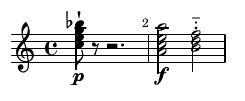
\includegraphics{Chords.png}

\begin{lstlisting}[language=XML, caption=Chord example]
      <note>
        <pitch>
          <step>B</step>
          <octave>4</octave>
        </pitch>
        <duration>4</duration>
        <voice>1</voice>
        <type>half</type>
        <notations>
          <articulations>
            <staccato />
            <detached-legato />
          </articulations>
        </notations>
      </note>
      <note>
        <chord />
        <pitch>
          <step>D</step>
          <octave>5</octave>
        </pitch>
        <duration>4</duration>
        <voice>1</voice>
        <type>half</type>
      </note>
      <note>
        <chord />
        <pitch>
          <step>F</step>
          <octave>5</octave>
        </pitch>
        <duration>4</duration>
        <voice>1</voice>
        <type>half</type>
      </note>
\end{lstlisting}
%\end{figure}

% -------------------------------------------------------------------------
\subsection{Tuplets}\label{tuplets}
% -------------------------------------------------------------------------

The situation for tuplets is different than that of the chords: there is a {'\tt <tuplet>}' element, with a {'\tt type}' attribute to indicate the note upon which it starts and stops:

\begin{lstlisting}[language=XML]
        <notations>
          <tuplet number="1" type="start" />
        </notations>
\end{lstlisting}

The {'\tt number}' attribute can be used to describe nested tuplets:

The contents, i.e. the notes in the tuplet, are not nested in the latter: there are placed in sequence between the two {'\tt <tuplet>}' elements that delimitate the tuplet. 

Each note in the tuplet has a {'\tt <time-modification>}' element, from the first one on. This element contains two elements:
\begin{lstlisting}[language=XML]
        <time-modification>
          <actual-notes>3</actual-notes>
          <normal-notes>2</normal-notes>
        </time-modification>
\end{lstlisting}

One should play {'\tt <actual-notes>}' within the time taken by only {'\tt <normal-notes>}'. The example above is thus that of a triplet.

In the case of {'\tt tuplets/Tuplets.xml}', shown below, the duration of the tuplets member is 20 quanta, i.e. 2/3 of a quarter note, whose duration is 30, and the 'display' duration is a quarter note. The duration of the triplet as a whole is that of a half note, i.e. 60 quanta.

%\begin{figure}
%\caption{First tuplet from {'\tt tuplets/Tuplet.xml}'}\label{tuplets}
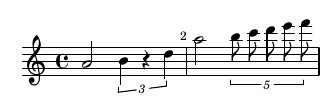
\includegraphics{Tuplet.png}

\begin{lstlisting}[language=XML, caption=Tuplet example]
        <divisions>30</divisions>

			<!-- ... ... ... ... ... -->
			
      <note>
        <pitch>
          <step>B</step>
          <octave>4</octave>
        </pitch>
        <duration>20</duration>
        <voice>1</voice>
        <type>quarter</type>
        <time-modification>
          <actual-notes>3</actual-notes>
          <normal-notes>2</normal-notes>
        </time-modification>
        <notations>
          <tuplet number="1" type="start" />
        </notations>
      </note>
      <note>
        <rest />
        <duration>20</duration>
        <voice>1</voice>
        <type>quarter</type>
        <time-modification>
          <actual-notes>3</actual-notes>
          <normal-notes>2</normal-notes>
        </time-modification>
      </note>
      <note>
        <pitch>
          <step>D</step>
          <octave>5</octave>
        </pitch>
        <duration>20</duration>
        <voice>1</voice>
        <type>quarter</type>
        <time-modification>
          <actual-notes>3</actual-notes>
          <normal-notes>2</normal-notes>
        </time-modification>
        <notations>
          <tuplet number="1" type="stop" />
        </notations>
      </note>
\end{lstlisting}
%\end{figure}

% -------------------------------------------------------------------------
% -------------------------------------------------------------------------
\section{Spanners}
% -------------------------------------------------------------------------
% -------------------------------------------------------------------------

% -------------------------------------------------------------------------
% -------------------------------------------------------------------------
\section{Barlines and repeats}
% -------------------------------------------------------------------------
% -------------------------------------------------------------------------

% -------------------------------------------------------------------------
% -------------------------------------------------------------------------
\section{Creating \mxml\ data}
% -------------------------------------------------------------------------
% -------------------------------------------------------------------------

This can be done in various ways:
\begin{itemize}
\item by hand, using a text editor: possible, but unrealistic for usual scores;
\item by exporting the score as an \mxml\ text file with a GUI music score editor;
\item by scanning a graphics files containing a ready-to-print score, with tools such as PhotoScore Ultimate\texttrademark;
\item by programming an application that outputs \mxml\ text.
\end{itemize}

This author has performed manual text editing on some of the samples supplied with {\tt libmusicxml2} in order to perform tests and debug {'\tt xml2ly}', but this is a particular case.

Exporting to \mxml\ is probably the most frequent way, and there are applications that do a good job at that. If an application supports say scordaturas in scores, then creating a {'\tt <scordatura>}' element is not very difficult.

Scanning graphical scores is a tough problem:  how do you tell lyrics from annotations such as {'\tt cresc.}' or tempos such as {'\tt Allegro}'? One usually has to manually fix scanning errors and the category of some text fragments after scanning to get good results. And, then, the scanning application should create quality \mxml\ data.

Creating \mxml\ by an application is a matter of computer programming, and requires development skill. As an example, {\tt libmusicxml2ly} supplies the necessary tools, and one can obtain:

\begin{lstlisting}[language=XML]
        <key>
          <fifths>1</fifths>
        </key>
\end{lstlisting}

with C++ code such as:

\begin{lstlisting}[language=XML]
  Sxmlelement attributes = factory::instance().create(k_attributes);

  Sxmlelement key = factory::instance().create(k_key);
  key->push (newElement(k_fifths, "1"));
  attributes->push (key);
\end{lstlisting}
 
% -------------------------------------------------------------------------
% -------------------------------------------------------------------------
\section{Importing \mxml\ data}
% -------------------------------------------------------------------------
% -------------------------------------------------------------------------

Many GUI applications provide a way to import \mxml\ data, often with some limitations. We show some of them here.

% -------------------------------------------------------------------------
\subsection{Small element, big effect}
% -------------------------------------------------------------------------

In {'\tt harmonies/Inversion.xml}', shown below, there is a harmony with an {'\tt <inversion>}' element. A number of applications ignore this element when importing \mxml\ data, because it takes a full knowledge of chords structures to compute the bass note of inverted chords.
%\begin{figure}
%\caption{Harmony inversion from {'\tt harmonies/Inversion.xml}'}\label{inversion}
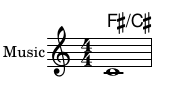
\includegraphics{Inversion.png}

\begin{lstlisting}[language=XML, caption = Harmony inversion]
      <harmony>
        <root>
          <root-step>F</root-step>
          <root-alter>1</root-alter>
        </root>
        <kind>major</kind>
        <inversion>2</inversion>
      </harmony>
\end{lstlisting}
%\end{figure}

% -------------------------------------------------------------------------
\subsection{Some elements often not well handled}
% -------------------------------------------------------------------------

There are elements that are not displayed in a "standard" way by the usual music score editors. One of them is the {'\tt <beat-repeat>}'.


% -------------------------------------------------------------------------
\subsection{Some elements usually not handled}
% -------------------------------------------------------------------------

There are elements that are not displayed by the usual music score editors, because there is no "standard" way to do so. One of them is the scordatura used on fretted string instrument.

For example, {'\tt strings/Scordatura.xml}' can be displayed like this using {\tt xml2ly} and LilyPond:

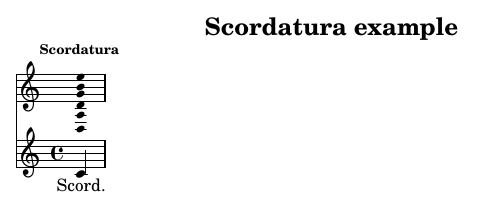
\includegraphics{Scordatura.png}

\begin{lstlisting}[language=XML, caption =Scordatura example]
          <scordatura>
              <accord string="6">
                <tuning-step>D</tuning-step>
                <tuning-alter>0</tuning-alter>
                <tuning-octave>3</tuning-octave>
              </accord>
              <accord string="5">
                <tuning-step>A</tuning-step>
                <tuning-alter>0</tuning-alter>
                <tuning-octave>3</tuning-octave>
              </accord>
              <accord string="4">
                <tuning-step>D</tuning-step>
                <tuning-alter>0</tuning-alter>
                <tuning-octave>4</tuning-octave>
              </accord>
              <accord string="3">
                <tuning-step>G</tuning-step>
                <tuning-alter>0</tuning-alter>
                <tuning-octave>4</tuning-octave>
              </accord>
              <accord string="2">
                <tuning-step>B</tuning-step>
                <tuning-alter>0</tuning-alter>
                <tuning-octave>4</tuning-octave>
              </accord>
              <accord string="1">
                <tuning-step>E</tuning-step>
                <tuning-alter>0</tuning-alter>
                <tuning-octave>5</tuning-octave>
              </accord>
          </scordatura>

\end{lstlisting}


% -------------------------------------------------------------------------
\subsection{A real challenge}
% -------------------------------------------------------------------------

The contents of {'\tt challenging/BeethovenNinthSymphony.xml}' is nearly 70 megabytes large. It was created by exporting it from Sibelius\texttrademark, and contains the whose score for this symphony. One can imagine the amount of work to create the score with a GUI in the first place, and, of course, there's no way a human could create such \mxml\ data by hand.

The reader is urged to try and import this file in their favorite score editing sofware. This author's experience is that:

\begin{itemize}
\item Finale\texttrademark 2014 finds it well-formed but too big to be opened;
\item MuseScore 3.3 opens it, but then working on the file is extremely slow;
\item musicxml2ly, supplied with LilyPond, converts it to LilyPond syntax as of 2.19.83, but with small issues that can be fixed.
\end{itemize}

% -------------------------------------------------------------------------
% -------------------------------------------------------------------------
\section{Conclusion}
% -------------------------------------------------------------------------
% -------------------------------------------------------------------------

There is a lot of information about \mxml\ on the Internet. And of course, plenty of targeted ready-to-use examples can be found at \url{https://github.com/grame-cncm/libmusicxml/tree/lilypond/files/samples/musicxml}.

\lstlistoflistings

%\listoffigures

\tableofcontents

% -------------------------------------------------------------------------
\end{document}
% -------------------------------------------------------------------------


%% -------------------------------------------------------------------------
%% hyperref
%% -------------------------------------------------------------------------
%
%\def\@StructureLinksColor{\ifx\isundefined \StructureLinksColor darkgray \else \StructureLinksColor\fi}
%
%\def\@URLColor{\ifx\isundefined \URLColor blue \else \URLColor\fi}
%
%\def\@PageLinksColor{\ifx\isundefined \PageLinksColor darkgray \else \PageLinksColor\fi}
%
%\def\@ContentsLinksColor{\ifx\isundefined \ContentsLinksColor purple \else \ContentsLinksColor\fi}
%
%\def\@TOCLinksColor{\ifx\isundefined \TOCLinksColor purple \else \TOCLinksColor\fi}
%
%
%\hypersetup{
%	colorlinks=true,
%	breaklinks=true,
%	linkcolor=\@StructureLinksColor,
%	urlcolor=\@URLColor,
%	pagecolor=\@PageLinksColor
%	}
%
%\newcommand{\ContentsLabel}[1]%
%	% Arguments: etiquette
%	{%
%	\hypertarget{#1}{\label{#1}}%
%	}
%
%\newcommand{\ContentsLink}[2]%
%	% Arguments: etiquette texteDuLien
%	{%
%	\hypersetup{linkcolor=\@ContentsLinksColor}%
%	\hyperlink{#1}{#2, voir page~\pageref{#1}~\includegraphics{MarquePourLiens}}%
%	\hypersetup{linkcolor=\@StructureLinksColor}%
%	}
%
%\newcommand{\ContentsPageLink}[2]%
%	% Arguments: etiquette texteDuLien
%	{%
%	\hypersetup{linkcolor=\@PageLinksColor}%
%	\hyperlink{#1}{#2 page~\pageref{#1}~\includegraphics{MarquePourLiens}}%
%	\hypersetup{linkcolor=\@StructureLinksColor}%
%	}
%
%\newcommand{\URL}[1]%
%	% Argument: l'URL
%	{{\footnotesize \url{#1}}}
%
%\newcommand{\RFC}[1]%
%	% Argument: numero de RFC
%	{%
%	\href{http://www.ietf.org/rfc/rfc#1.txt}{RFC~#1~ \includegraphics{MarquePourLiens}}%
%	}
